\section{Accelerator Design} \label{sec:gun_design}

The acceleration region of our prototype UEM system has several requirement which are unique in comparison to standard electron guns.
Primarily, given the limitations on the beam discussed earlier, %TODO link to discussion of Childs law beam size limitation
the employ laser pulse must be a relatively large area.
This concern leads to several additional criteria.
To accomodate this large beam, the anode aperture must be similarly large; in fact, this will be larger than the emission source due to beam expansion during acceleration.
Also, in transit from the cathode to the anode, this large beam is more susceptable to non-uniformities in the accelerating electic field given that it will span a wider proportion of the accelerator than thin beams used in standard TEM.

\begin{figure}
  \centering
  \begin{tikzpicture}
  \node at (0,0) {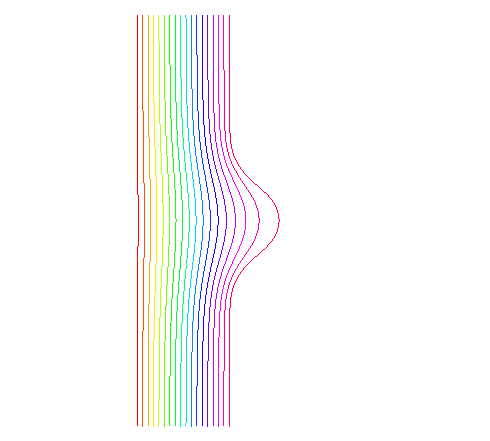
\includegraphics{gunfield.png}};
  \draw [fill=blue!40]
    (-1.4,-3.1)
    -- ++(0,6.2)
    -- ++(-1.1,0)
      node [above, pos=0.5] {$-V$}
    -- ++(0,-6.2)
      node [right=0.5, rotate=90, pos=0.7] {Photocathode}
    -- cycle
  ;
  \fill
    (-1.4,-0.4)
    -- ++(0,0.8)
      coordinate [pos=0.5] (source)
    -- ++(-0.1,0)
    -- ++(0,-0.8)
    -- cycle
  ;
  \draw [fill=blue!40, radius=0.7]
    (-0.15,-2.45)
    -- ++(0,1.35)
    arc [start angle=180, end angle=90]
    -- ++(0.4,0)
    -- ++(0,-2.75)
    -- ++(-0.4,0)
    arc [start angle=270, end angle=180]
    -- cycle
  ;
  \draw [fill=blue!40, radius=0.7]
    (-0.15,1.1)
    -- ++(0,1.35)
    arc [start angle=180, end angle=90]
    -- ++(0.4,0)
      node [pos=0.1,above] {$0V$}
    -- ++(0,-2.75)
    -- ++(-0.4,0)
    arc [start angle=270, end angle=180]
    -- cycle
  ;
  \draw [green, <-, ultra thick]
    (source)
    -- ++(-70:4)
      node [black,right] {Laser}
  ;
\end{tikzpicture}

  \caption{
    Schematic of the employed Togawa inspired cathode ($-V$) and anode (0V) pair.
    The emission source is inserted behind the cathode Wehnelt.
    Also shown are simulated equipotential lines generated by FEM modeling.
    The separation of the cathode and anode is adjustable to allow a greater range of input laser angles if needed. 
  }
  \label{fig:gun-field}
\end{figure}

These requirements lead to the fabrication of cathode/Wehnelt and anode pair based on the design of Togawa \textit{et al.} \cite{togawa_ceb6_2007}.
A schematic of this design, overlayed by a Finite Element Model (FEM) simulation of the electic field, is shown in \ref{fig:gun-field}.
The schematic shows that the aperture concerns are easily satisfied.
From the field equipotentials, it is clear that this design has a consistently flat electric field for large displacements off the central axis.

%TODO comment on alignment
%TODO comment on high voltage
%TODO comment on EV parts etc
